\chapter{Wi-Fi Protected Access (WPA)}
\label{ch:wpa}

\section{WPA Einführung}
Das \gls{wpaLabel} Protokoll wurde als notwendiger Nachfolger des \gls{wepLabel} Protokolls definiert.
Zur selben Zeit war der weiterführender, sehr umfangreichen Standard \textit{\gls{ieeeLabel} 802.11i} in Arbeit, der aber zum Zeitpunkt als \gls{wepLabel} geknackt wurde noch nicht abgeschlossen war.
So wurden Anfangs 2003 die ersten zertifizierten \gls{wpaLabel}-fähigen \gls{wlanLabel}-Geräte auf den Markt gebracht.
Seit September 2004 gibt es zertifizierte \gls{wpa2Label} Netzwerkgeräte. Das \gls{wpa2Label} Protokoll entspricht nun dem \textit{\gls{ieeeLabel} 802.11i} Standard.
\gls{wpaLabel} nutzt das \gls{tkipLabel} zur Verschlüsselung, während \gls{wpa2Label} den \gls{aesLabel} verwendet.\footcite{Wi-Fi_Protected_Access__Wikipedia_2015-04-10}\footcite{WPA2__Wikipedia_2015-04-10}

\subsection{Sicherheit}
Das \gls{wpa2Label} Protokoll gilt bis heute als sicher und sollte als einziges verwendet werden.

Da \gls{wpaLabel} und \gls{wpa2Label} sehr viele Ähnlichkeiten aufweisen, wird folgend der Begriff \gls{wpaLabel} übergreifend für beide Standards verwendet. Bei Differenzen wird die jeweilige Version explizit bezeichnet.

Ein erfolgreicher Angriff kann bisher nur via \gls{glos:bruteforceLabel}- und Wörterbuch-Angriff erfolgen, was relativ unmöglich ist, vorausgesetzt es wird ein \textit{sicherer} \gls{pskLabel} verwendet.

\todo{Box mit sicherem Passwort:  (mind. 16 zufälligen alphanumerischen Zeichen)}

Die ganze Sicherheit basiert auf dem \gls{pskLabel}.
Sobald der bekannt ist, kann eine Kommunikation problemlos mitgehört werden.
Sprich trotz einem sicheren Schlüssel, kann jeder Netzteilnehmer aktive Verbindungen der anderen abhören, insofern die nicht andersartig verschlüsselt werden (z.B. mit \gls{httpsLabel}).


\subsection{Authentifizierungs-Varianten}
\gls{wpaLabel} bietet nebst der \gls{pskLabel} Methode (die auch als \textit{\gls{wpaLabel}-Personal} bekannt ist), auch eine \textit{enterprise} Methode an.
Dabei wird ein Authentifizierung-Server verwendet, der jeden Nutzer einzeln authentifiziert und für jede Sitzung einen neuen \gls{pmkLabel} generiert.
Das \textit{enterprise} Protokoll wird oft in Firmen angewendet, lohnt sich jedoch für den privaten Gebrauch nicht, da der Einrichtungsaufwand und Betrieb eines eigenen Servers zu hoch ist.
Deshalb wird in dieser Arbeit auf die \gls{pskLabel} Methode eingegangen.


\subsubsection{WPS Standard}
Der \gls{wpsLabel} Standard entspricht keiner konkreten Zugriffsmethode, sondern soll das Einrichten von sicheren \gls{pskLabel} clientseitig erleichtern.

Dazu gibt es folgende vier Methoden:\footcite{Wi-Fi_Protected_Setup_-_Wikipedia_the_free_encyclopedia_2015-04-10}
\begin{itemize}
	\item \textbf{PIN:} Ein 8-stelliger PIN des einen Gerätes muss auf dem anderen eingegeben werden.
	\item \textbf{Push button:} Per Kopfdruck am \gls{apLabel} wird eine zweiminütige Beitrittsphase des Netzwerkes gestartet.
	\item \textbf{\gls{nfcLabel}:} Die Daten werden via \gls{nfcLabel} ausgetauscht (was nur innerhalb kurzer Distanz möglich ist).
	\item \textbf{\gls{usbLabel}:} Die Netzinformationen werden via externen \gls{usbLabel} Storage ausgetauscht.
\end{itemize}

Die PIN Methode gilt als besonders unsicher, da lediglich eine 7-stellige Zahl erraten werden muss (die letzte entfällt, da sie einer Checksumme entspricht).
Als Gegenmassnahme kann (und soll) eine automatische zeitliche Sperre nach fehlgeschlagenen Versuchen eingestellt werden.\footcite{viehboeck_wps_2015-04-10}

\textit{Push button} und \textit{\gls{nfcLabel}} sind anfällig auf ungewollte Nutzer, wenn der \gls{apLabel} an einem unbewachten Ort steht und sich so jemand selbst authentifizieren kann.


\subsection{Schlüsselaustausch}
Voraussetzung für den gewöhnlichen Schlüsselaustausch ist der Besitz des \gls{pskLabel}.
Dieser Schlüssel kann aus 8 bis 63 druckbaren \gls{asciiLabel} Zeichen bestehen.

\subsubsection{Four-Way Handshake}
%\begin{wrapfigure}{r}{0.5\textwidth}
%	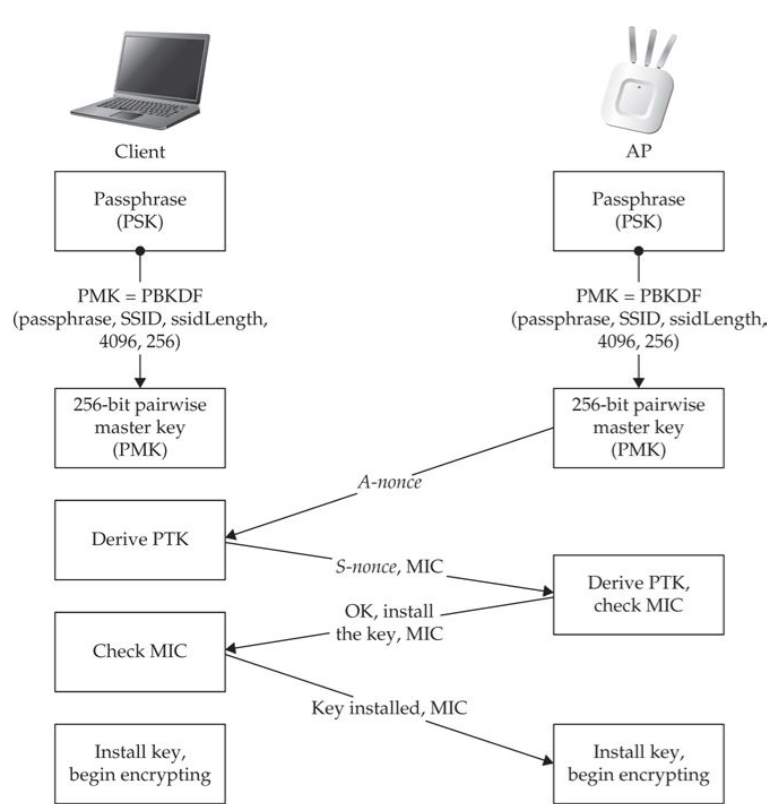
\includegraphics[width=1.0\linewidth]{images/wpa/four-way-handshake.png}
%	\caption[WPA: The four-way handshake]{WPA: \textit{The four-way handshake} (Quelle: \cite[][151]{WrightCache201503})}
%\end{wrapfigure}
\begin{figure}[H]
	\centering
	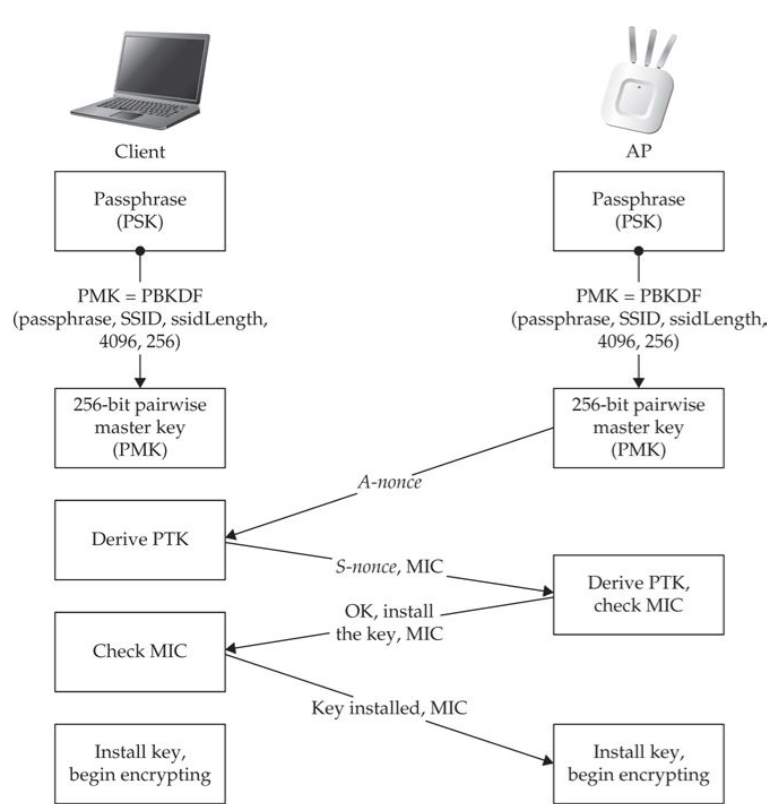
\includegraphics[width=0.8\linewidth]{images/wpa/four-way-handshake.png}
	\caption[WPA: The four-way handshake]{WPA: \textit{The four-way handshake} (Quelle: \cite[][151]{WrightCache201503})}
\end{figure}
Der \textit{Four-Way Handshake} bezeichnet den Zugriff eines Clients auf das Netzwerk.
Bei einer Verbindung zum Netzwerk wird beidseitig aus dem \gls{pskLabel} und der \gls{ssidLabel} der \gls{pmkLabel} berechnet.
Dafür wird 4096 mal ein \gls{hmacshaLabel} des \gls{pskLabel} berechnet. (Diese Berechnungen machen einen \gls{glos:bruteforceLabel}-Angriff so aufwändig.)
Der \gls{apLabel} überträgt dem Client eine zufällige Zahl (\textit{A-nonce}), welche der Client mit einer weiteren zufälligen Zahl (\textit{B-nonce}) ergänzt.
Der \gls{apLabel} berechnet aus den zufälligen Zahlen und den beiden \gls{macLabel}-Adressen einen temporären \gls{ptkLabel}, der pro Session neu generiert wird. Der \gls{ptkLabel} wird zudem auch während einer Session periodisch ausgetauscht.\footcite[][40f.]{WrightCache201503}

%\begin{figure}[H]
%	\centering
%	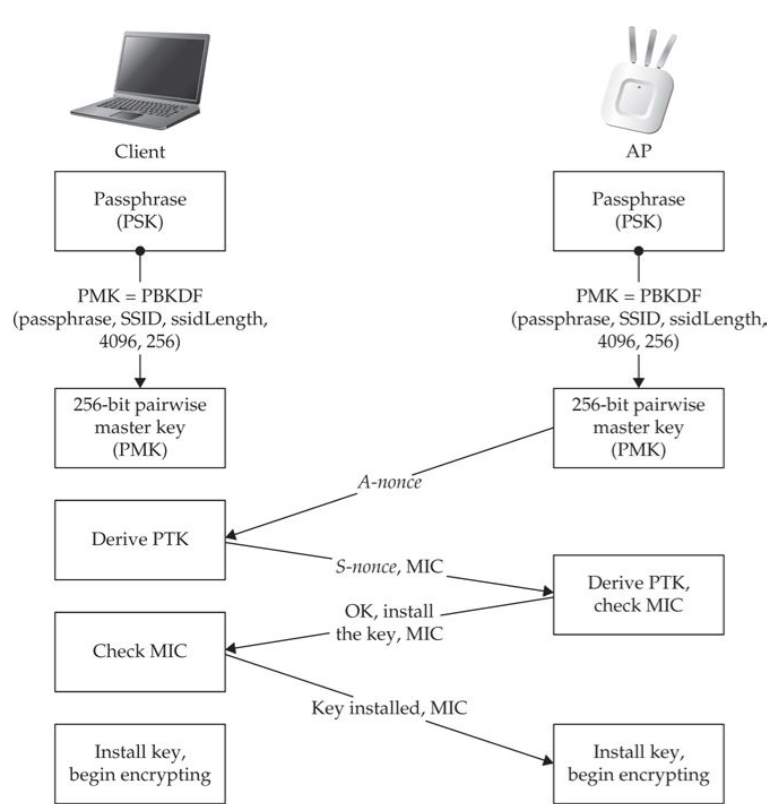
\includegraphics[width=0.6\linewidth]{images/wpa/four-way-handshake.png}
%	\caption[WPA: The four-way handshake]{WPA: \textit{The four-way handshake} (Quelle: \fullcite[][151]{WrightCache201503})}
%\end{figure}

Um einen Schlüssel zu knacken werden zusammengefasst folgende Informationen gebraucht:
\begin{itemize}
	\item Netzwerk \gls{ssidLabel}
	\item \textit{A-nonce}
	\item \textit{B-nonce}
	\item \gls{macLabel}-Adresse des Clients
	\item \gls{macLabel}-Adresse des \gls{apLabel}'s
	\item \gls{micLabel}: entspricht dem Hash der Nutzdaten. Dieser wird als korrekt verschlüsselte Nachricht verwendet. Sprich beim Ausprobieren der möglichen Schlüssel, kommt mit dem gesuchten \gls{pskLabel} derselbe \gls{micLabel}-Wert zustande.
\end{itemize}

Nebst während dem \textit{Four-Way Handshake}, werden diese Information auch regelmässig wiederholt.
So muss nicht zwingend ein vollständiger \textit{Four-Way Handshake} vorliegen.


\section{Angriff auf WPA}

\subsection{Angriffsmethode}
Für einen erfolgreichen Angriff müssen mindestens zwei Teile eines \textit{Four-Way Handshake} vorliegen.
Dazu müssen die Aktivitäten eines Channel, wie im \cref{subsec:wep_crack_tutorial} wird, abgehört und gespeichert werden (z.B. mit \textit{airport}).

Falls sich keine Clients neu anmelden, können wie folgt bestehende Clients rausgeschmissen werden:
\begin{lstlisting}[style=lstStyleFramed]
aireplay-ng --deauth 1 -a A4:52:6F:8A:9F:01 -c 2c:f0:ee:20:7c:32 en0
\end{lstlisting}
\begin{tabular}{l l}
	\textbf{Parameter} & \textbf{Bedeutung}\\
	-{}-deauth 1 & löst einmal 64 Deauthentifizierungs-Pakete aus\\
	-a	& \gls{macLabel}-Adresse des \gls{apLabel}\\
	-c	& \gls{macLabel}-Adresse des Client\\
	en0 & zu verwendendes \gls{glos:interfaceLabel}
\end{tabular}

\subsection{Bruteforce}
\todo{Bruteforce bei glossary ergänzen}
Der Rest des Angriffes kann offline erfolgen. Durch Ausprobieren wird nach einem gültigen \gls{pskLabel} gesucht, der einen gültigen \gls{micLabel}-Hash berechnet. Dies wird für alle möglichen Schlüssel durchprobiert.
Es gibt verschiedene Programme die den \gls{glos:bruteforceLabel} durchführen können.
Einige davon sind im \cref{subsec:wpa_attack_tutorial} dokumentiert.

Die Berechnung ist je nach Schlüssellänge und bekannten Schlüsselinformationen sehr intensiv und wird daher oft statt von der \gls{cpuLabel}, von der \gls{gpuLabel}, sprich der Grafikkarte, ausgerechnet.
Ausserdem kann die Berechnung anstatt von einem \textit{\gls{glos:onPremiseLabel}} Rechner, in der \textit{"`\gls{glos:cloudLabel}"'} ausgeführt werden.

Damit nicht alle mögliche Kombinationen, die aus den druckbaren \gls{asciiLabel} Zeichen erstellt werden können, durchprobiert werden müssen, werden oft nur Wörter aus einem definierten Wörterbuch probiert.
Manche Programme unterstützen auch Passwortmasken, durch die nebst der Schlüssellänge auch pro Zeichenposition eine Auswahl an Zeichen definiert werden kann. So kann die Rechenzeit bei genügend Informationen erheblich reduziert werden.


\subsection{Konkreter Angriff auf ein WPA-Netzwerk}
\label{subsec:wpa_attack_tutorial}

In diesem \cref{subsec:wpa_attack_tutorial} basieren viele Inhalte auf dem Buch "`Hacking Exposed Wireless"'.\footcite[][148f.]{WrightCache201503}

\subsubsection{Testumgebung}
\label{subsubsec:wpa_test_environment}

Folgend wird das \gls{wpa2Label}-Testnetz mit der \gls{ssidLabel} \textit{YHX-02427} als Angriffsziel verwendet.
Das Netz wird durch den aktuellen Swisscom-Router \textit{Centro grande} zur Verfügung gestellt. \footcite{Centro_grande_Analog_Standard_-_WLAN_Router_Swisscom_2015-04-15}

Die Konfiguration, unter anderem die \gls{ssidLabel} und der \gls{pskLabel}, entsprechen dem Auslieferungszustandes.
Darum sind folgende Eigenschaften des \gls{pskLabel}'s im Vorhinein bekannt:
\begin{itemize}
	\item Der \gls{pskLabel} besteht aus vier-mal-vier Zeichen getrennt durch ein "`-"' (Minus). Sprich die Länge beträgt total 19 Zeichen, wovon drei bereits bekannt sind (die Minuszeichen).
	\item Eine vierstellige Zeichenfolge besteht ausschliesslich aus Kleinbuchstaben und Zahlen.
\end{itemize}

Es werden drei verschiedene Programme (\textit{crack utilities}) verwendet:
%\footcite{Aircrack-ng_2015-04-06}
%\footcite{pyrit_Google_Project_Hosting_2015-04-13}
%\footcite{hashcat_advanced_password_recovery_2015-04-13}
\begin{table}[H]
% style
\small\sffamily\centering\renewcommand{\arraystretch}{1.4}
% caption
\captionabove{Verwendete Programme}
%tabular
\rowcolors{1}{tablebodycolor}{tablerowcolor}
\begin{tabular}{l l l}
\hline
\rowcolor{tableheadcolor}
  \bfseries Name  &
  \bfseries Version(en) &
  \bfseries Link \\
\hline
  \textbf{aircrack-ng} & 1.1, 1.2\_rc2 & \url{http://www.aircrack-ng.org/}\\
  \textbf{pyrit} & 0.4.0 & \url{https://code.google.com/p/pyrit/}\\
  \textbf{hashcat} & 0.49 & \url{http://hashcat.net/hashcat}\\
\hline
\end{tabular}
\end{table}


\subsubsection{Datenbereinigung}
Angenommen ein gültiger \textit{Four-Way Handshake} wurde aufgezeichnet, entfernen wir mit \textit{pyrit} alle überflüssigen Daten aus dem \textit{capture}:
\begin{lstlisting}[style=lstStyleFramed]
pyrit -r YHX-02427_raw.cap -o YHX-02427.cap strip
\end{lstlisting}
Anschliessend wird man aufgefordert die gewünschte \gls{ssidLabel} auszuwählen.
Bei meinen Tests schrumpften Dateien von 20\,MB auf 8\,KB.
Übrig bleiben nur noch die Handshakes von \gls{wpaLabel} und die \gls{ivLabel}'s von \gls{wepLabel}.

\subsubsection{Aircrack-ng Bruteforce}
Anschliessend kann bereits ein \textit{aircrack-ng} \gls{glos:bruteforceLabel}-Angriff ausgeführt werden:
\begin{lstlisting}[style=lstStyleFramed]
aircrack-ng YHX-02427.cap -w wordlist.txt -b A4:52:6F:8A:9F:01
\end{lstlisting}
\begin{tabular}{l l}
	\textbf{Parameter} & \textbf{Bedeutung}\\
	*.cap & \textit{capture}-Datei mit mind. einem Handshake\\
	-w	& Textdatei mit allen zu probierenden \gls{pskLabel}'s (einer pro Zeile)\\
	-b	& \gls{bssidLabel} des \gls{apLabel}\\
\end{tabular}

\subsubsection{Pyrit Bruteforce}
Alternativ kann mit \textit{pyrit} ebenfalls ein \gls{glos:bruteforceLabel}-Angriff durchgeführt werden:
\begin{lstlisting}[style=lstStyleFramed]
pyrit -r YHX-02427.cap -i wordlist.txt -b a4:52:6f:8a:9f:01 attack_passthrough
\end{lstlisting}
\begin{tabular}{l l}
	\textbf{Parameter} & \textbf{Bedeutung}\\
	-r & \textit{capture}-Datei mit mind. einem Handshake\\
	-i	& Textdatei mit allen zu probierenden \gls{pskLabel}'s (einer pro Zeile)\\
	-b	& \gls{bssidLabel} des \gls{apLabel}\\
	attack\_passthrough & definiert, dass ausgerechnete Hashes nicht zwischengespeichert werden\\
\end{tabular}


\subsubsection{Hashcat Bruteforce}
Um mit \textit{hashcat} einen \gls{glos:bruteforceLabel}-Angriff durchzuführen, muss die \textit{.cap} Datei in eine \textit{.hccap} Datei umgewandelt werden. Dies kann mit \textit{aircrack-ng} erledigt werden.

\begin{lstlisting}[style=lstStyleFramed]
./aircrack-ng -J YHX-02427 YHX-02427.cap
\end{lstlisting}
\begin{tabular}{l l}
	\textbf{Parameter} & \textbf{Bedeutung}\\
	-J & \gls{ssidLabel} des Netzwerkes\\
	*.cap & \textit{capture}-Datei mit mind. einem Handshake\\
\end{tabular}

\begin{framed}
	\textbf{Bemerkung:} Dazu wird allerdings die neuste \textit{aircrack-ng} Version \textit{"`1.2-rc2"'} benötigt, welche nicht in \textit{Homebrew} vorhanden ist und daher selbst kompiliert werden muss. Die Installation ist auf der \textit{aircrack-ng} Website beschrieben.\\
	Trotzdem, dass beim Kompilieren Fehler angezeigt werden, befindet sich anschliessend ein lauffähige \textit{aircrack-ng} Datei im \textit{src} Ordner, mit der die \textit{.hccap} Datei generiert werden kann.
\end{framed}

Es wird eine neue Datei mit \textit{[\gls{ssidLabel}].hccap} erstellt. Im konkreten vorliegenden Beispiel also: \textit{YHX-02427.hccap}.

Nebst dem wird der \textit{A-nonce ("`anonce"')} , \textit{B-nonce ("`snonce"')}und der \textit{\gls{micLabel} ("`Key MIC"')} angezeigt.
\begin{figure}[H]
	\centering
	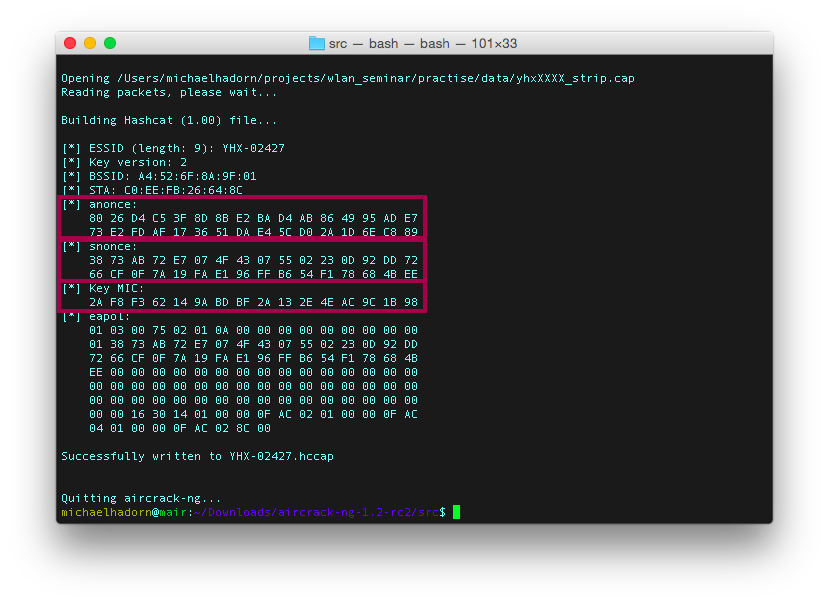
\includegraphics[width=0.9\textwidth]{images/wpa/conversion_cap2hccap.png}
	\caption{Strip capture -- \textit{aircrack-ng}}
\end{figure}

Wie bisher können wir erneut einen Wörterbuch-Angriff starten:
\begin{lstlisting}[style=lstStyleFramed]
hashcat -m 2500 YHX-02427.hccap wordlist.txt
\end{lstlisting}
\begin{tabular}{l l}
	\textbf{Parameter} & \textbf{Bedeutung}\\
	-m & Hash Type (2500 = \gls{wpaLabel}/\gls{wpa2Label}) (\textit{hashcat -h} um alle anzuzeigen)\\
	*.hccap & \textit{capture}-Datei mit mind. einem Handshake\\
	*.txt & Textdatei mit allen zu probierenden \gls{pskLabel}'s (einer pro Zeile)\\
\end{tabular}

Zudem kann \textit{hashcat} auch Passwörter mit Platzhalter knacken:\footcite{mask_attack_hashcat_wiki_2015-04-13}
\begin{lstlisting}[style=lstStyleFramed]
hashcat -m 2500 -a 3 --pw-min=19 --pw-max=19 YHX-02427.hccap -1 ?l?d ?1?1?1?1-?1?1?1?1-?1?1?1?1-?1?1?1?1
\end{lstlisting}
\begin{tabular}{l l}
	\textbf{Parameter} & \textbf{Bedeutung}\\
	-m & Hash Type (2500 = WPA/WPA) (\textit{hashcat -h} um alle anzuzeigen)\\
	-a 3 & \textit{Attack mode} (3 = Bruteforce)\\
	-{}-pw-min/max & min. und max. Länge des \gls{pskLabel}\\
	*.hccap & \textit{capture}-Datei mit mind. einem Handshake\\
	-1 & Pattern mit alphanumerisch (nur Kleinbuchstaben \textit{?l} und Zahlen \textit{?d})\\
	$[mask]$ & Passwort Maske (mit zuvor definiertem Pattern (\textit{-1}))\\
\end{tabular}

Folgende Ausgabe erscheint: (mit \textit{enter} kann jeweils eine Statusmeldung erzeugt werden)
\begin{figure}[H]
	\centering
	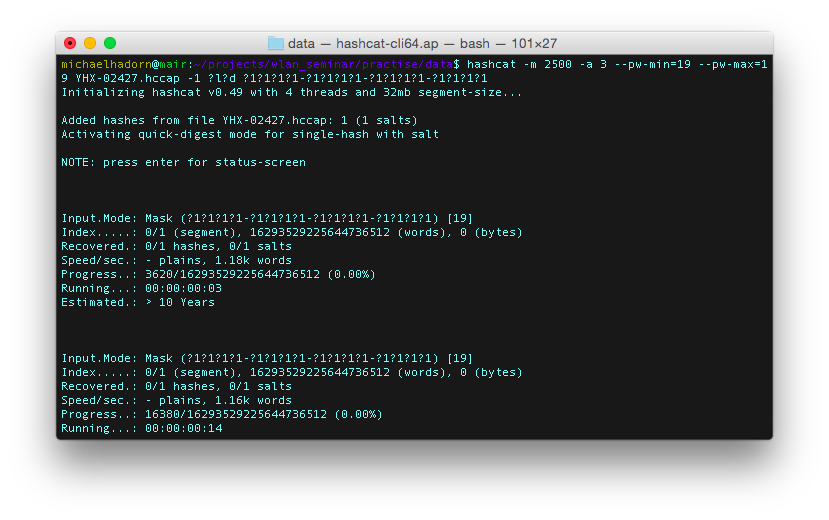
\includegraphics[width=0.9\textwidth]{images/wpa/hashcat_bruteforce_pattern.png}
	\caption{\textit{hashcat} \gls{glos:bruteforceLabel} mit Passwortmaske -- \textit{aircrack-ng}}\label{fig:hashcat_bruteforce_pattern}
	\floatfoot{\textbf{Bemerkung zur obriger \cref{fig:hashcat_bruteforce_pattern}:} Dem sehr aufmerksamen Leser fällt auf, dass die Anzahl der Worte (\textit{words}) nicht korrekt ist. Dies ist mit hoher Wahrscheinlichkeit auf ein programminterner \textit{Overflow} zurückzuführen, da die Angaben für kleinere Passwörter korrekt sind.\\
	Die korrekte Anzahl zu testende Worte wäre um den Faktor $10^5$ grösser.
	Anstatt die gegebenen $1.63 * 10^{19}$ ist $ 36^{16} = 7.96 * 10^{24} $ korrekt.}
\end{figure}

Obwohl wir relativ viele Informationen zum \gls{pskLabel} besitzen und die Länge nicht übermässig lang gewählt ist, werden wir höchstwahrscheinlich den \gls{pskLabel} nicht herausfinden.


\subsubsection{Sicherheit und Rechenzeit}

Basierend auf den bekannten Passwortinformationen aus \cref{subsubsec:wpa_test_environment} kommen für jedes der 16 unbekannten Zeichen 26 Buchstaben oder 10 Zahlen zur Auswahl.

\begin{equation}
	\begin{split}
	\label{eqn:wpa_attack_key_possibelities}
	P_{Anzahl\,Möglichkeiten} &= n_{Anzahl\,Zeichen}\,^{p_{Anzahl\,Positionen}}\\
	&= 36^{16} = 7.9587 * 10^{24}
	\end{split}
\end{equation}

Aus \cref{fig:hashcat_bruteforce_pattern} ist die Geschwindigkeit $v_{speed} = 1.18k\,hashes/sec$ ersichtlich.
(Falls alle anderen Programme auf dem System geschlossen werden, steigt die Geschwindigkeit leicht auf $v_{speed} = 1.23k\,hashes/sec$ an.
Für folgende Berechnungen wurde die gewöhnliche Geschwindigkeit $v_{speed} = 1.18k\,hashes/sec$ verwendet.)

Daraus kann die Dauer des Angriffes wie folgt berechnet werden:
\begin{equation}
	\begin{split}
	\label{eqn:wpa_attack_duration_hours}
	T_{years} &= P_{Anzahl\,Möglichkeiten} / v_{speed} / t_{minLen} / t_{hourLen} / t_{dayLen} / t_{yearLen}\\
	&= 36^{16} / 1180 / 60 / 60 / 24 / 365 = 2.1387 * 10^{14}\,Jahre
	\end{split}
\end{equation}

\cref{eqn:wpa_attack_duration_hours} verdeutlicht die Sicherheit des Passwortes. Würde man alle Möglichkeiten ausprobieren dauert der Angriff 213 Billionen Jahre.

Bekannterweise hängt die Rechenzeit stark von der Schlüssellänge ab.
Folgende \cref{fig:wpa_attack_linear} und \cref{fig:wpa_attack_log} veranschaulichen jene Abhängigkeit, basierend auf den Kriterien des zu knackenden Schlüssels.

\begin{figure}[H]
	\begin{minipage}[b]{.45\linewidth}
	   	\pgfplotsset{width=1.0\textwidth, height=0.7\textwidth}
		\centering
		\begin{tikzpicture}
			\begin{axis}[
				xlabel={$x$ = Passwortlänge},
				ylabel={$t_R$ = \textbf{Stunden}}
			]
				\addplot[draw=blue][domain=0:4.8]{(36^x) / 1180 / 60 / 60};
			\end{axis}
		\end{tikzpicture}
		\subcaption{Rechenzeit in \textbf{Stunden}}\label{fig:1a}
	\end{minipage}%
	\begin{minipage}[b]{.45\linewidth}
		\pgfplotsset{width=1.0\textwidth, height=0.7\textwidth}
		\centering
		\begin{tikzpicture}
			\begin{axis}[
				xlabel={$x$ = Passwortlänge},
				ylabel={$t_R$ = \textbf{Jahre}}
			]
				\addplot[draw=blue][domain=0:7.6]{(36^x) / 1180 / 60 / 60 / 24 / 365};
			\end{axis}
		\end{tikzpicture}
		\subcaption{Rechenzeit in \textbf{Jahren}}\label{fig:1b}
	\end{minipage}
	\caption{Rechenzeit \textbf{linear} in Abhängigkeit der Passwortlänge}\label{fig:1}
	\label{fig:wpa_attack_linear}
\end{figure}

\begin{figure}[H]
	\begin{minipage}[b]{.65\linewidth}
		\pgfplotsset{width=1.0\textwidth, height=0.7\textwidth}
		\centering
		\begin{tikzpicture}
			\begin{axis}[
				xlabel={$x$ = Passwortlänge},
				ylabel={$t_R$ = \textbf{Jahre \textit{log.}}},
				ymode = log,
			]
				\addplot[draw=blue][domain=5:60]{(36^x) / 1180 / 60 / 60 / 24 / 365};
			\end{axis}
		\end{tikzpicture}
	\end{minipage}
	\caption{Rechenzeit \textbf{logarithmisch} in Abhängigkeit der Passwortlänge in \textbf{Jahren}}\label{fig:}
	\label{fig:wpa_attack_log}
\end{figure}


\subsubsection{Verbesserungsmöglichkeiten und Beschleunigungen}
Lässt man anstelle der \gls{cpuLabel} die \gls{gpuLabel} die Hashes berechnen, erreicht man abhängig der Grafikkarte 40'000 bis 60'000 hashes/sec. Dies entspricht ungefähr einer 50-fachen Beschleunigung.\footcite[][158]{WrightCache201503}

Da das Aufwändige des Angriffes die Berechnung der Hashes ist, können alternativ bereits ausgerechnete \glspl{glos:rainbowTableLabel} verwendet werden.
Abhängig der Hardware können so 200'000'000\,hashes/sec getestet werden. Dies wiederum entspricht gegenüber dem traditionellen \gls{cpuLabel} Angriff eine 200'000-fache Beschleunigung.\footcite[][160]{WrightCache201503}
%176,830,746 PMK/second
Die Hashes von \gls{wpaLabel} beinhalten jedoch als \gls{glos:saltLabel} die \gls{ssidLabel}, sprich die \glspl{glos:rainbowTableLabel} können nur für Netze mit der selben \gls{ssidLabel} verwendet werden, was die Nutzung erheblich einschränkt.


\subsubsection{Fazit des Angriffes}
Schlussendlich folgt, dass für \gls{wpaLabel} trotz massiver Beschleunigung von bis zu 50-facher (oder sogar 200'000-facher mit \glspl{glos:rainbowTableLabel}) die durchschnittliche Knackzeit des Swisscom Router \gls{pskLabel}'s via \gls{glos:bruteforceLabel} nicht während Lebenszeiten abgeschlossen werden kann.

Wenn wir die benötige Rechenzeit mit der durchschnittlichen Einsatzdauer eines Routers vergleichen, erkennt man, dass die \gls{pskLabel}-Länge mit mehr als genügender Sicherheit gewählt wurde.

Die Sicherheit gilt solange kein anderer Weg als ein \gls{glos:bruteforceLabel}-Angriff bekannt ist.
